\documentclass[
  bibliography=totoc,     % Literatur im Inhaltsverzeichnis
  captions=tableheading,  % Tabellenüberschriften
  titlepage=firstiscover, % Titelseite ist Deckblatt
]{scrartcl}

% Paket float verbessern
\usepackage{scrhack}

% Warnung, falls nochmal kompiliert werden muss
\usepackage[aux]{rerunfilecheck}

% unverzichtbare Mathe-Befehle
\usepackage{amsmath}
% viele Mathe-Symbole
\usepackage{amssymb}
% Erweiterungen für amsmath
\usepackage{mathtools}

% Fonteinstellungen
\usepackage{fontspec}
% Latin Modern Fonts werden automatisch geladen
% Alternativ:
%\setromanfont{Libertinus Serif}
%\setsansfont{Libertinus Sans}
%\setmonofont{Libertinus Mono}
\recalctypearea % Wenn man andere Schriftarten gesetzt hat,
% sollte man das Seiten-Layout neu berechnen lassen

% deutsche Spracheinstellungen
\usepackage{polyglossia}
\setmainlanguage{german}


\usepackage[
  math-style=ISO,    % ┐
  bold-style=ISO,    % │
  sans-style=italic, % │ ISO-Standard folgen
  nabla=upright,     % │
  partial=upright,   % ┘
  warnings-off={           % ┐
    mathtools-colon,       % │ unnötige Warnungen ausschalten
    mathtools-overbracket, % │
},                       % ┘
]{unicode-math}

% traditionelle Fonts für Mathematik
\setmathfont{Latin Modern Math}
% Alternativ:
%\setmathfont{Libertinus Math}

\setmathfont{XITS Math}[range={scr, bfscr}]
\setmathfont{XITS Math}[range={cal, bfcal}, StylisticSet=1]

% Zahlen und Einheiten
\usepackage[
locale=DE,                   % deutsche Einstellungen
separate-uncertainty=true,   % immer Fehler mit \pm
per-mode=symbol-or-fraction, % / in inline math, fraction in display math
]{siunitx}

% chemische Formeln
\usepackage[
version=4,
math-greek=default, % ┐ mit unicode-math zusammenarbeiten
text-greek=default, % ┘
]{mhchem}

% richtige Anführungszeichen
\usepackage[autostyle]{csquotes}

% schöne Brüche im Text
\usepackage{xfrac}

% Standardplatzierung für Floats einstellen
\usepackage{float}
\floatplacement{figure}{htbp}
\floatplacement{table}{htbp}

% Floats innerhalb einer Section halten
\usepackage[
section, % Floats innerhalb der Section halten
below,   % unterhalb der Section aber auf der selben Seite ist ok
]{placeins}

% Seite drehen für breite Tabellen: landscape Umgebung
\usepackage{pdflscape}

% Captions schöner machen.
\usepackage[
  labelfont=bf,        % Tabelle x: Abbildung y: ist jetzt fett
  font=small,          % Schrift etwas kleiner als Dokument
  width=0.9\textwidth, % maximale Breite einer Caption schmaler
]{caption}
% subfigure, subtable, subref
\usepackage{subcaption}

% Grafiken können eingebunden werden
\usepackage{graphicx}
% größere Variation von Dateinamen möglich
\usepackage{grffile}

% schöne Tabellen
\usepackage{booktabs}

% Verbesserungen am Schriftbild
\usepackage{microtype}

% Literaturverzeichnis
\usepackage[style=alphabetic,]{biblatex}
% Quellendatenbank
\addbibresource{lit.bib}

% Hyperlinks im Dokument
\usepackage[
  unicode,        % Unicode in PDF-Attributen erlauben
  pdfusetitle,    % Titel, Autoren und Datum als PDF-Attribute
  pdfcreator={},  % ┐ PDF-Attribute säubern
  pdfproducer={}, % ┘
]{hyperref}
% erweiterte Bookmarks im PDF
\usepackage{bookmark}

% Trennung von Wörtern mit Strichen
\usepackage[shortcuts]{extdash}

\title{V703: Das Geiger-Müller-Zählrohr}
\author{
  Simon Schulte
  \texorpdfstring{
    \\
    \href{mailto:simon.schulte@udo.edu}{simon.schulte@udo.edu}
  }{}
  \texorpdfstring{\and}{, }
  Tim Sedlaczek
  \texorpdfstring{
    \\
    \href{mailto:tim.sedlaczek@udo.edu}{tim.sedlaczek@udo.edu}
  }{}
}
\publishers{TU Dortmund – Fakultät Physik}

\date{Durchführung: 18.04.2017\\
      Abgabe: 25.04.2017}


\begin{document}

\maketitle
\thispagestyle{empty}
\tableofcontents
\newpage
\section{Theorie}
\label{sec:theorie}
In diesem Versuch wird das Geiger-Müller-Zählrohr untersucht. Das
Geiger-Müller-Zählrohr dient dazu, die Intensität ionisierender Strahlung zu
messen. Wenn nämlich ionisierende Strahlung in das Geiger-Müller-Zählrohr
eintritt, gibt das Zählrohr einen elektronischen Impuls ab, welcher leicht von
einem Impulsmesser wahrgenommen werden kann.
In Abbildung \ref{fig:V7031} zu sehen ist der schematische Aufbau eines
solchen Zählrohrs. Ein Zählrohr besteht aus einem Stahlmantel, in dessen
Mitte sich axial ein positiv geladener Anodendraht befindet. Der Anodendraht
leitet widerum die Betriebsspannung $U$. Diese ist nötig, um eine
Potentialdifferenz zwischen dem Mantel und dem Draht zu gewährleisten. Außerdem
ist eine Mylar-Folie am linken Ende des Zählrohrs befestigt, welche als
Eintrittsfenster dient. Diese gewährleistet, dass sogar $\alpha$-Strahlung in
das Rohr durchdringt, welche eigentlich schon von einem Stück Papier aufgehalten
wird. In diesem Versuch wird allerdings nur $\beta$-Strahlung (in Form von Elektronen) betrachtet. Im
Inneren des Zählrohrs ist ein Gasgemisch, welches hauptsächlich aus Argon besteht. Das Gasgemisch hat den Zweck, dass,
wenn ein geladenes Teilchen durch das Eintrittsfenster dringt, sich dieses so
lange durch das Gasgemisch bewegt, bis dessen Energie durch Ionisationskontakte
aufgebraucht ist.
\begin{figure}[htb]
  \centering
  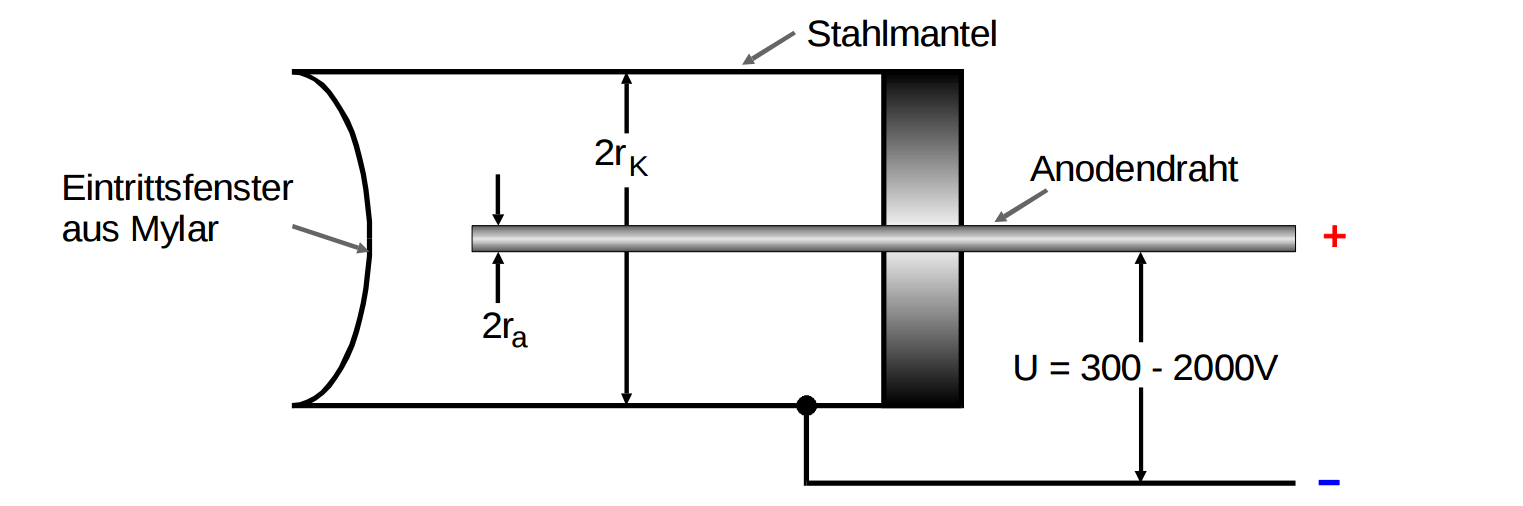
\includegraphics[width=0.9\textwidth]{V7031.png}
  \caption{Der Querschnitt eines Endfenster-Zählrohrs}
  \label{fig:V7031}
\end{figure}
In Abbildung \ref{fig:V7032} zu sehen ist nun die Abhängigkeit der Anzahl der
erzeugten Ionenpaare von der Spannung $U$ bei einem Proportionalitätszählrohr.
So werden bei kleinen Betriebsspannungen nur wenige Elektronen den Draht
erreichen, da die meisten vorher rekombiniert werden. Diese erste Zone wird
Rekombination der Sammlung genannt. In der zweiten Zone, der
Ionisationskammer, können aufgrund der immer größer werdenden Spannung kaum noch
Elektronen rekombinieren, bevor sie den Anodendraht erreichen können. Damit
kommen fast alle Elektronen am Draht an. Diese erzeugen dann einen
Ionisationsstrom, der proportional zur Energie der ionisierenden Strahlung ist.
In der dritten Zone, dem (begrenzten) Proportionalbereich entsteht Stoßionisation.
Das heißt, dass die Elektronen bei den Zusammenstößen mit dem Gasgemisch
hinreichend viel Energie aufnehmen, um selbst ionisieren zu können. Da sich diese
Elektronen selbst immer wieder ionisieren können, nimmt deren Anzahl lawinenartig
zu, auch Townsend-Lawine genannt. In der vierten Zone beginnt dann der
Arbeitsbereich des Geiger-Müller-Zählrohrs, gennant Auslösebereich. Die
Elektronenlawinen breiten sich nun nicht mehr nur, wie in Zone 3, in Feldrichtung
aus, sondern längst des gesamten Drahtes. Dadurch entstehen elektrische
Impulse, die dann groß genug sind, um sie mit einem Impulszähler zu detektieren.
\begin{figure}[htb]
  \centering
  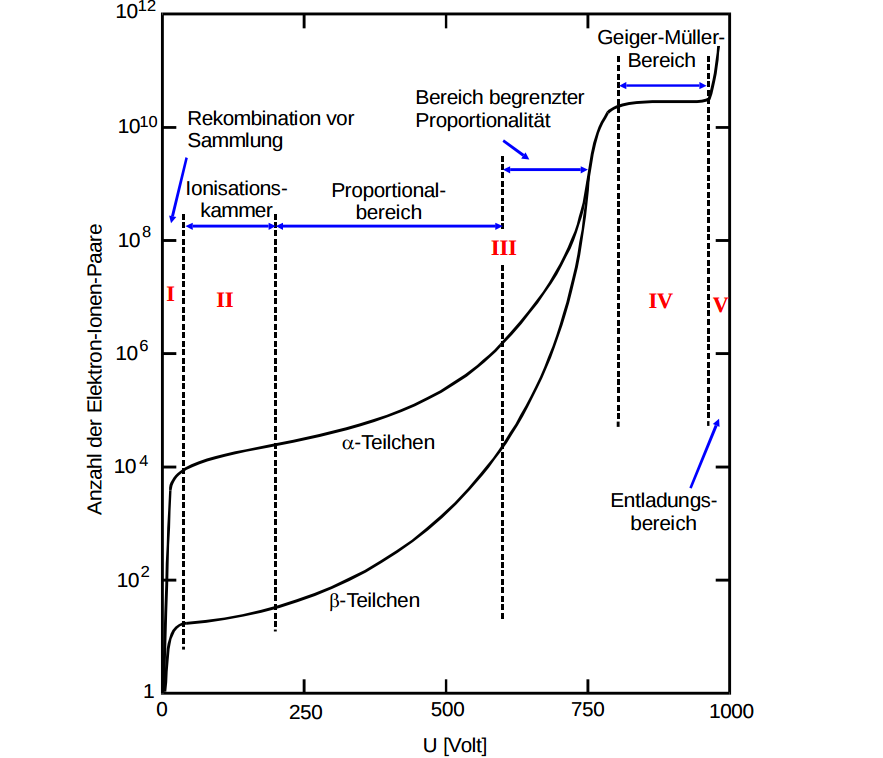
\includegraphics[width=0.9\textwidth]{V7032.png}
  \caption{Die Anzahl der erzeugten Elektron-Ionenpaare [n] als Funktion der
  Spannung U [V] bei einem Proportionalzählrohr}
  \label{fig:V7032}
\end{figure}
In Abbildung \ref{fig:V7033} zu sehen ist nun die Tot- und Erholzeit des
Zählrohrs, wobei die Ladung als Funktion der Zeit dargestellt wird.
Es bildet sich zunächst durch die positiven Ionen ein Ionenschlauch in dem
Zählrohr. Da Protonen eine 1836-mal größere Masse als Elektronen haben
verschwinden diese auch langsamer. Damit bleibt dieser Ionenschlauch länger
bestehen und baut ein Gegenfeld zum E-Feld auf, was dazu führt, dass das
Zählrohr in der Totzeit keine weitere $\beta$-Strahlung detektiert.
Nach der Totzeit stellt sich die Erholungszeit ein, in welcher widerum die
abgegebenen elektrischen Impulse des Rohrs kleiner ausfallen.
\begin{figure}[htb]
  \centering
  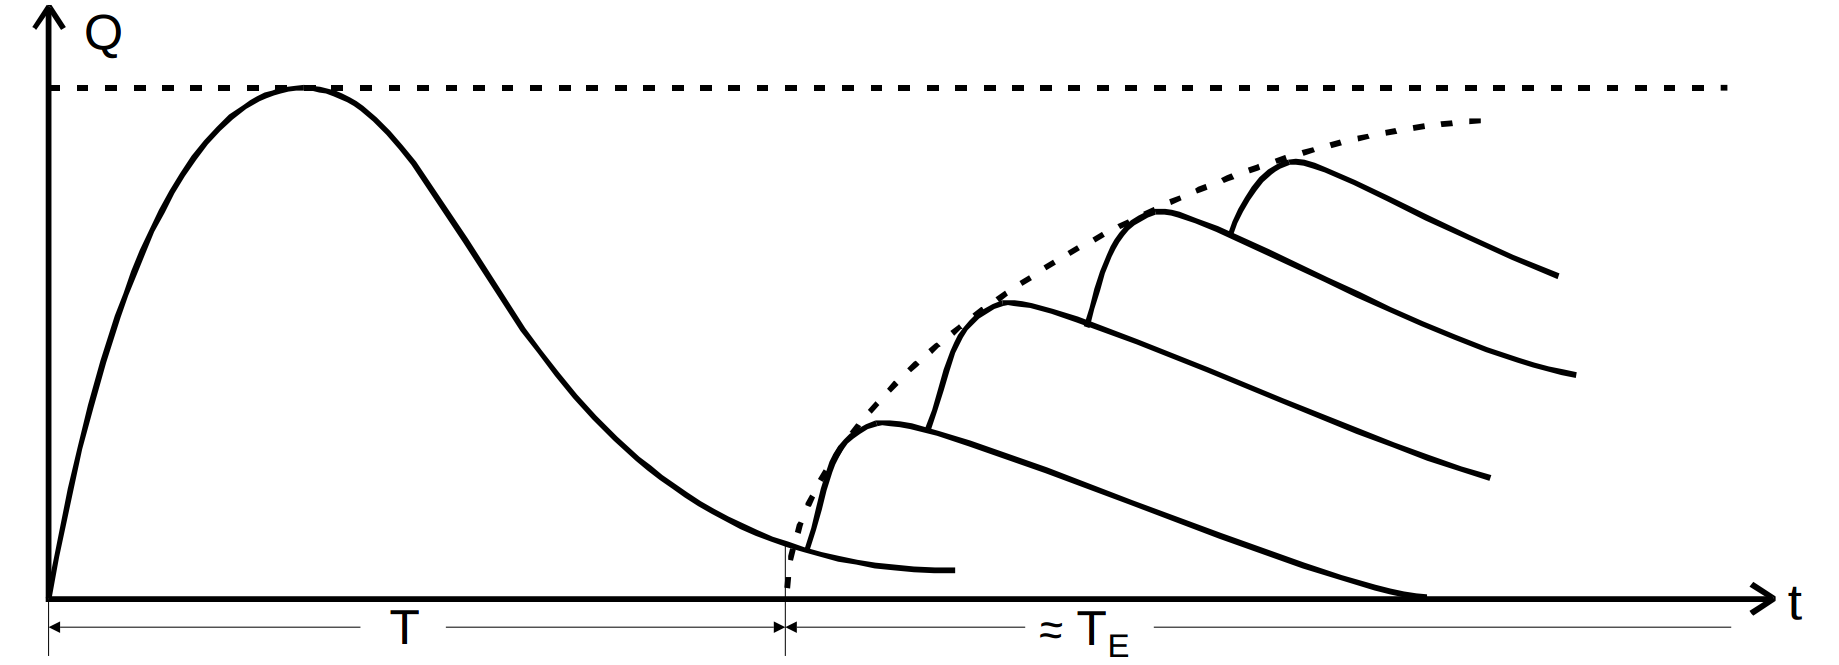
\includegraphics[width=0.9\textwidth]{V7033.png}
  \caption{Die Tot- und Erholungszeit eines Zählrohrs, dabei wird die Ladung [Q]
  als Funktion der Zeit abgebildet.}
  \label{fig:V7033}
\end{figure}
In Abbildung \ref{fig:V7034} zu sehen ist die Charakteristik eines Zählrohres.
Die Charakteristik trägt die Spannung $U$ gegen die im Zählrohr registrierte
Teilchenzahl $N$ auf. Dabei wird eine konstante $\beta$-Strahlungsquelle verwendet.
Besonders interessant ist dabei das Plateau, welches in einem idealen Zählrohr
konstant wäre, aber aufgrund von Nachentladungen in der Realität leicht ansteigt.
Diese Nachentladungen entstehen, wenn die positiv geladenen Ionen große Energien
erreichen. Wenn sie dann an den Stahlmantel gelangen sind sie in der Lage
Elektronen aus dem Stahlmantel zu lösen. Dadurch wird die Messung verfälscht.
Dem wird entgegengewirkt, indem dem Zählrohrgasgemisch Alkohol hinzugegeben wird.
Alkoholmoleküle sind vielkettig und die überflüssige Energie der Ionen kann
somit in Form von Schwingungsenergie an die langen Alkoholmoleküle abgegeben werden.
Allerdings klappt dies auch nicht einwandfrei, weshalb sich eben diese
Charakteristik, mit einem nicht perfekten, nicht geraden Plateau, ergibt.
\begin{figure}[htb]
  \centering
  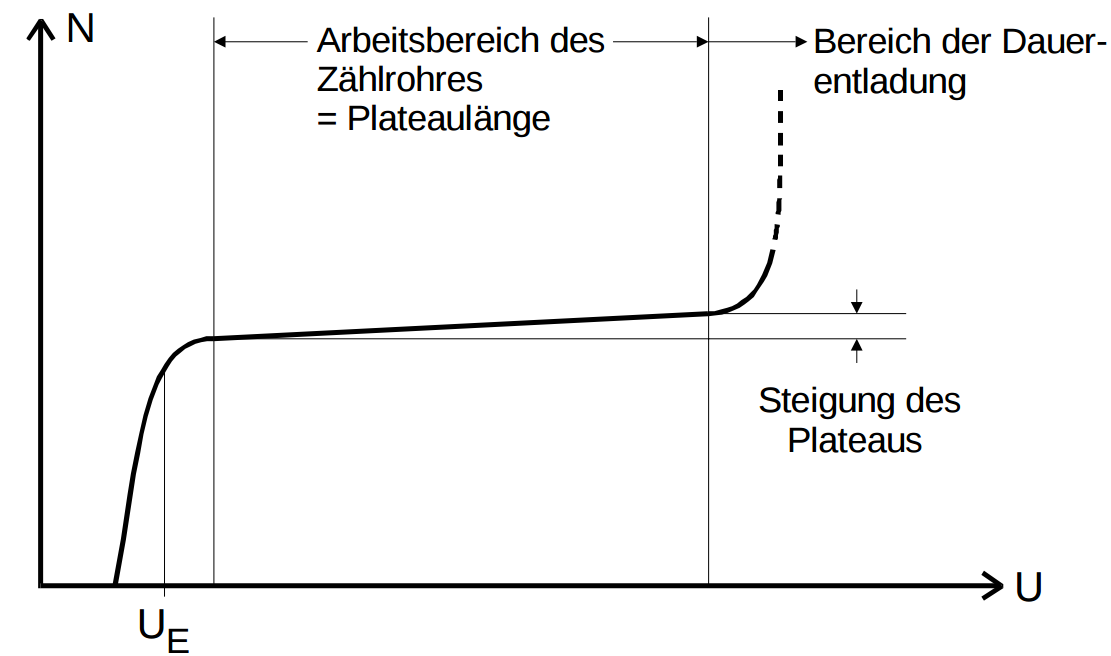
\includegraphics[width=0.9\textwidth]{V7034.png}
  \caption{Die Charakteristik eines Zählrohres.}
  \label{fig:V7034}
\end{figure}
\section{Durchführung}
\subsection{Versuchsaufbau}
\begin{figure}[htb]
  \centering
  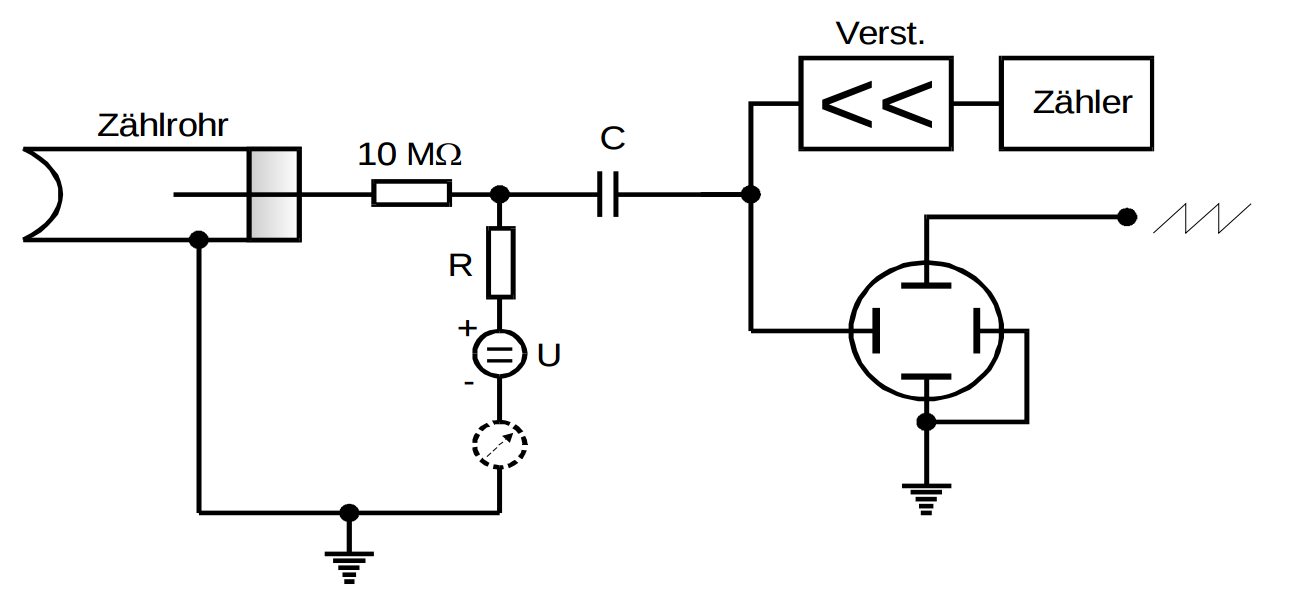
\includegraphics[width=0.9\textwidth]{V7035.png}
  \caption{Die Skizze der Messapparatur.}
  \label{fig:V7035}
\end{figure}
In Abbildung \ref{fig:V7035} zu sehen ist der Versuchsaufbau. Links ist das
Geiger-Müller-Zählrohr, mit dem Zähldraht, der mit einem
elektrischen Stromkreis verbunden ist. Die Ladungen der Elektronen werden dabei
auf dem Zähldraht gesammelt, um dann über den Widerstand $R$ zu fließen
und einen Spannungsimpuls zu verursachen. Dieser wird am Kondensator
ausgekoppelt und im Verstärker verstärkt. Der Zähler zählt dann die Anzahl
der Elektronen. Das Oszilloskop wird zur Visualisierung genutzt.
\subsection{Versuchsablauf}
In Teil a) soll eine Zählrohr-Charakteristik erstellt werden. Dafür wird eine
$\beta$-Strahlungsquelle vor dem Mylar-Eintrittsfenster platziert. Die
Charakteristik beinhaltet dann die Zählrate $n$ in Abhängigkeit von der
Betriebsspannung $U$ und der mit einem Mikro-Ampere-Meter gemessene Zählerstrom $I$.
Dann wird für die Werte \SI{320}{\volt} bis \SI{700}{\volt} in zehner Schritten
jeweils für 60 Sekunden die Zählrate gemessen. Damit wird der statistische
Fehler $\leq$ \SI{1}{\percent}.
In Teil b) wurden die beiden Nachentladungen für die Maximalspannung von
\SI{700}{\volt} bestimmt. Der Nachladeimpuls wurde am Oszilloskop abgelesen.
In Teil c) wurden bei verschiedenen Spannungen die Totzeiten und Erholungszeiten
bestimmt. Dabei wurden Spannungen zwischen \SI{400}{\volt} und \SI{500}{\volt}
gemessen, die in der Mitte des Plateaus liegen.
In Teil d) wurde bei einer Spannung von \SI{450}{\volt} (Plateaumitte) die
Anzahl der $N$ Teilchen von 2 verschiedenen $\beta$-Strahlern gemessen. Dabei
wurden 3 Messungen durchgeführt. Jeweils eine für die einzelnen Strahler und eine
für beide Strahler gleichzeitig.
\end{document}
